\documentclass{article}
\usepackage[utf8]{inputenc}
\usepackage{graphicx}
\usepackage{fancyhdr}
\usepackage{listings}
\usepackage{color}
\usepackage{hyperref}
\usepackage{amsmath}
\usepackage{amssymb}
\usepackage{subcaption}
\usepackage[total={6in, 9in}]{geometry}



\graphicspath{ {images/} }

\pagestyle{fancy}



\title{%
    Advanced High Performance Computing \\
    \vspace{0.4cm}
    \large Lecture Notes
}

\author{jerakrs}
\date{February 2018}


\begin{document}

\maketitle

\begin{abstract}
    This document is the lecture note of \textit{Advanced High Performance Computing}. The course code is \textit{COMS30006} and the unit director is \textit{McIntosh Smith}.
\end{abstract}


\section{BlueCrystal Phase 4}

Phase 4 (bc4login.acrc.bris.ac.uk) is primarily intended for large parallel jobs and for work requiring the Nvidia P100 GPUs. The \href{https://www.acrc.bris.ac.uk/acrc/index.htm}{\textcolor{blue}{home page}} can get more infomations about BlueCrystal Phase 4 and the
 \href{https://www.acrc.bris.ac.uk/protected/bc4-docs/index.html}{\textcolor{blue}{BlueCrystal Phase 4 User Documentation}} is the document of BlueCrystal Phase 4.


\section{Lattice Boltzmann}

Lattice Boltzmann methods (LBM) (or thermal Lattice Boltzmann methods (TLBM)) is a class of computational fluid dynamics (CFD) methods for fluid simulation. The \href{https://github.com/UoB-HPC/advanced-hpc-lbm}{\textcolor{blue}{first assigment}} is using MPI to improve the Lattice Boltzmann algorithm.


\subsection{Data Structure}

The 'speeds' in each cell are numbered as follows:
\begin{lstlisting}
                                6 2 5
                                 \|/
                                3-0-1
                                /|\
                                7 4 8
\end{lstlisting}

A 2D grid:
\begin{lstlisting}
                            cols
                        --- --- ---
                       | D | E | F |
                 rows  --- --- ---
                       | A | B | C |
                       --- --- ---
\end{lstlisting}

'unwrapped' in row major order to give a 1D array:
\begin{lstlisting}
                  --- --- --- --- --- ---
                 | A | B | C | D | E | F |
                  --- --- --- --- --- ---                      
\end{lstlisting}

Grid indicies are:
\begin{lstlisting}[language=C]
                          
                  ny
                  ^       cols(ii)
                  |  ----- ----- -----
                  | | ... | ... | etc |
                  |  ----- ----- -----
         rows(jj) | | 1,0 | 1,1 | 1,2 |
                  |  ----- ----- -----
                  | | 0,0 | 0,1 | 0,2 |
                  |  ----- ----- -----
                  ----------------------> nx
\end{lstlisting}


\subsection{Basic Code Structure}

\begin{itemize}
    \item initialise()
    \item for each timestep:
    \begin{itemize}
        \item accelerate flow()
        \item propagate()
        \item rebound()
        \item collision()
        \item av\_velocity()
    \end{itemize}
    \item write\_values()
    \item finalise()
\end{itemize}

\textbf{Initialise} function will load params, allocate memory, load obstacles and initialise fluid particle densities.

\textbf{Accelerate flow} will modify one row of cells, add to the right pointing speeds and subtract from the left pointing speeds.

\begin{figure}[h]
    \centering
    \begin{subfigure}{0.45\textwidth}
    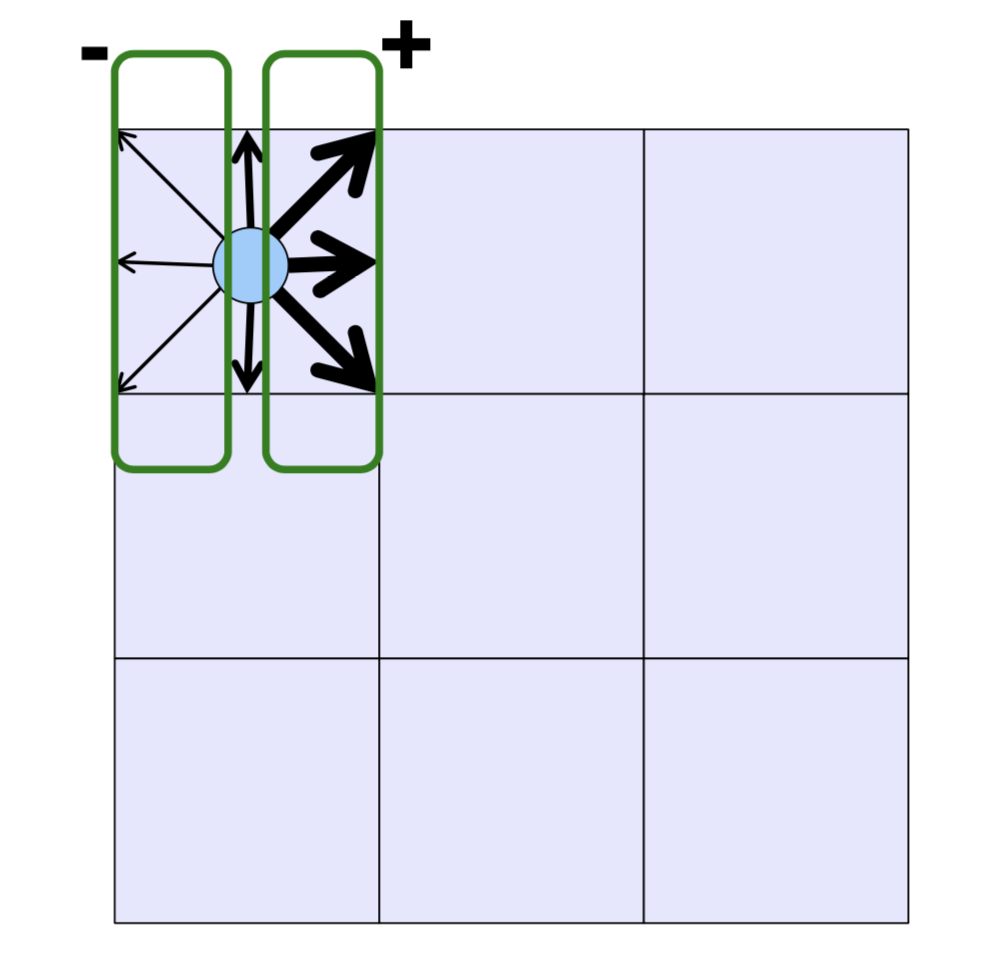
\includegraphics[scale=0.15]{images/accelerate_flow.png} 
    \caption{Accelerate Flow}
    \label{fig:my_label}
    \end{subfigure}
    \begin{subfigure}{0.45\textwidth}
    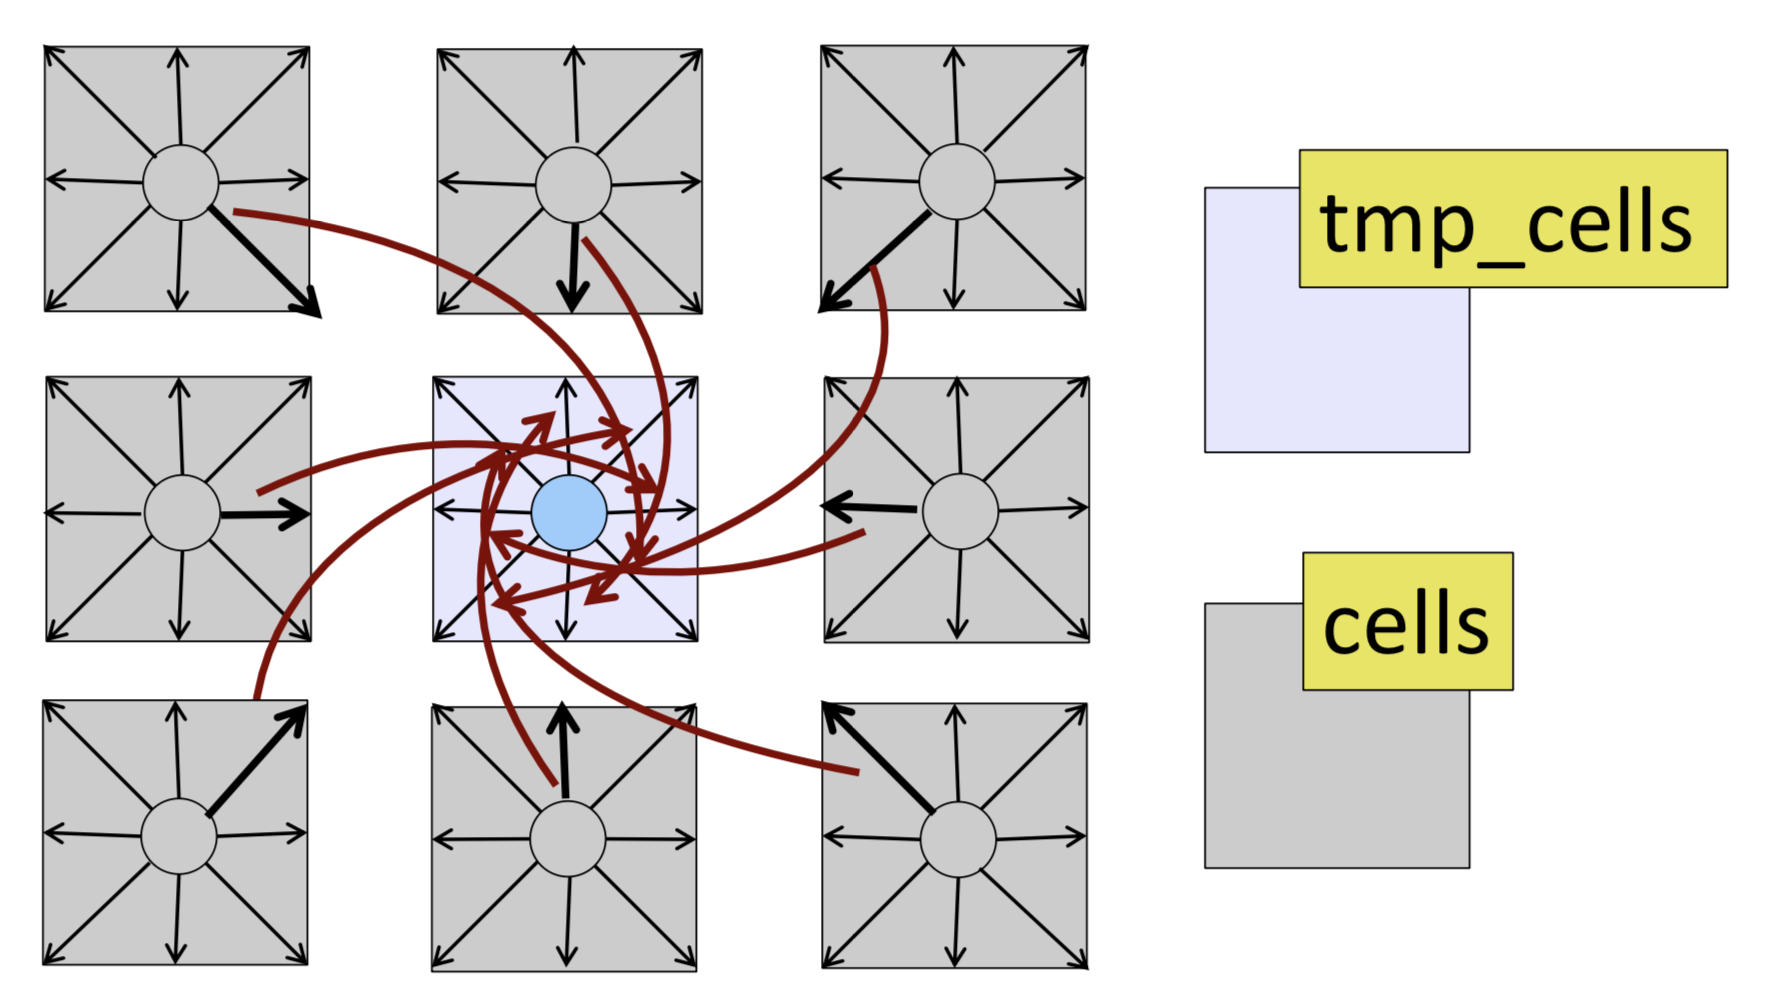
\includegraphics[scale=0.15]{images/propagation.png}
    \caption{Propagation}
    \label{fig:my_label}
    \end{subfigure}
\end{figure}


\textbf{Propagation}, after a time interval, each particle will move to the neighboring node in its direction.

\textbf{Rebound}, for obstacle cells, it will mirror the speeds in each cell.

\begin{figure}[h]
    \centering
    \begin{subfigure}{0.45\textwidth}
    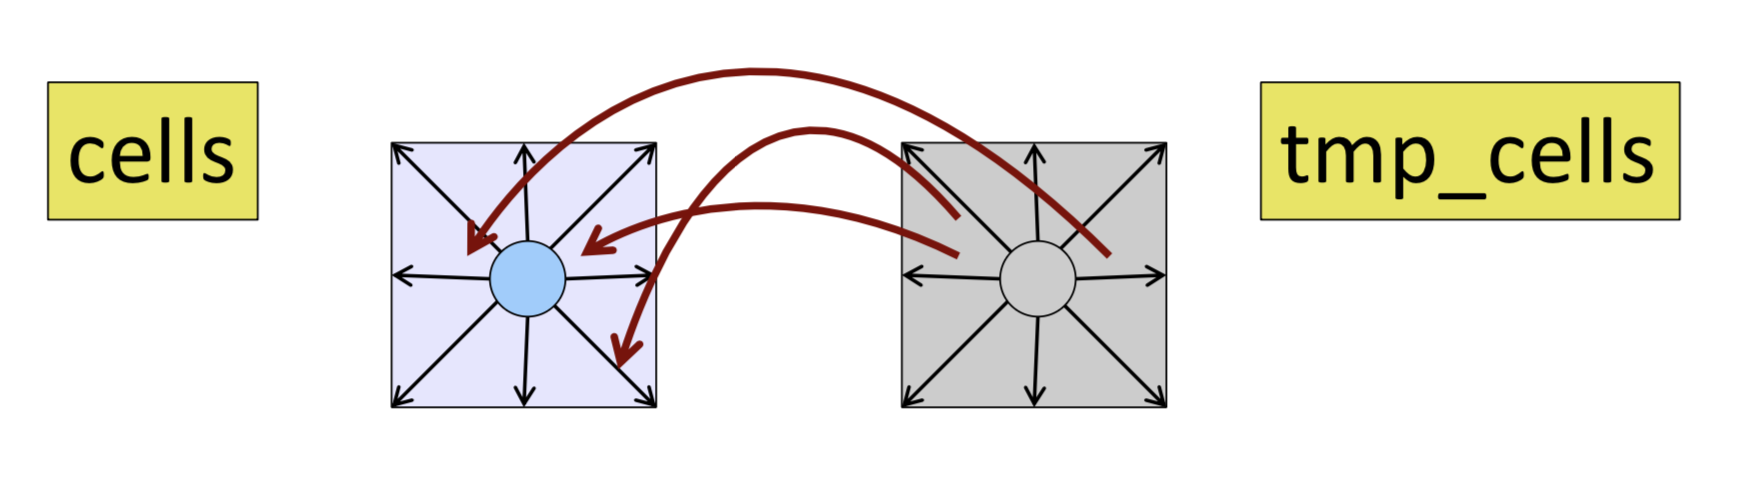
\includegraphics[scale=0.15]{images/rebound.png} 
    \caption{Rebound}
    \label{fig:my_label}
    \end{subfigure}
    \begin{subfigure}{0.45\textwidth}
    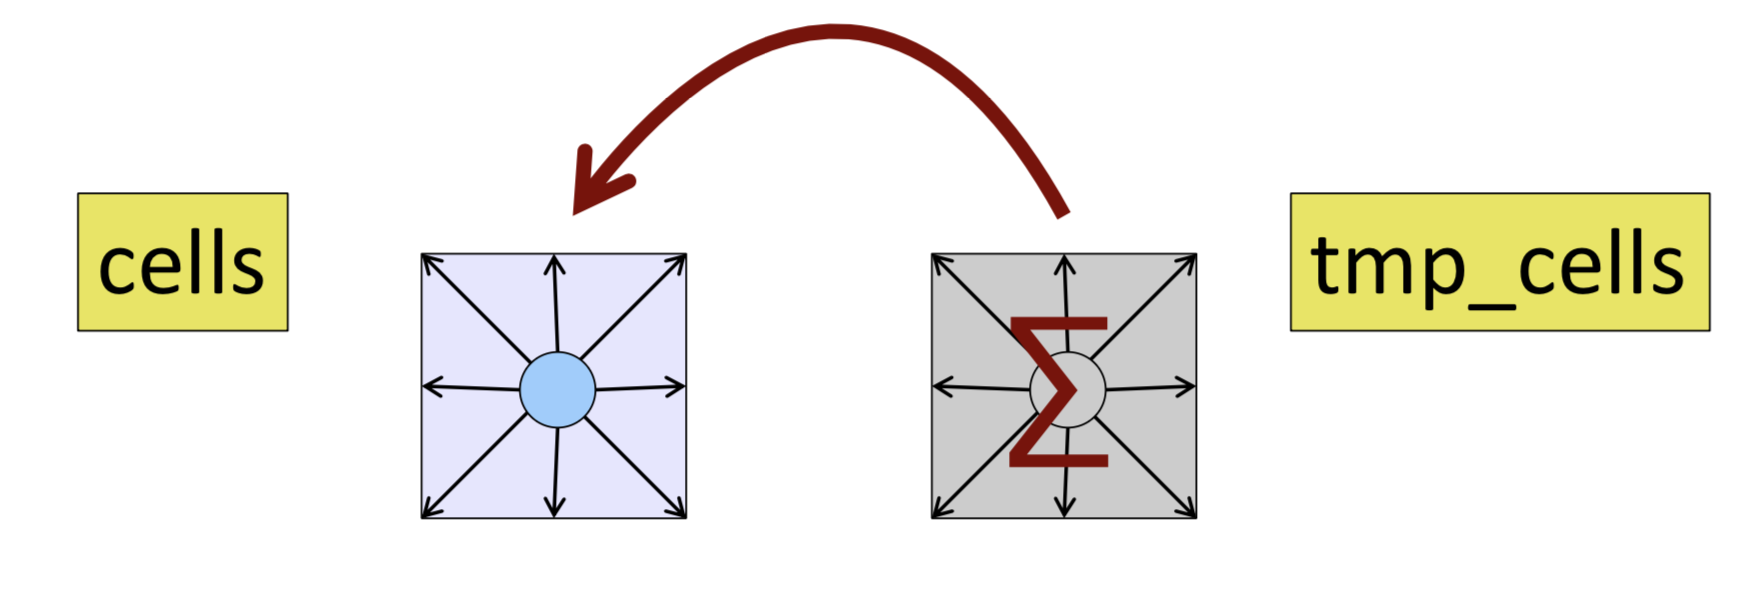
\includegraphics[scale=0.15]{images/collision.png}
    \caption{Collision}
    \label{fig:my_label}
    \end{subfigure}
\end{figure}

\textbf{Collision}, for non-obstacle cells, it will perform ’relaxation’ arithmetic in each cell.


\section{MPI-3}

\subsection{Domain Decomposition}

Decompose by columns, rows, tiles.

\subsection{Communication Pattern}

\textbf{MPI\_Send} and \textbf{MPI\_Recv} is asynchronous when there is a system buffer, but blocking if copying large messages into a buffer since its own overheads.

\textbf{MPI\_Isend} and \textbf{MPI\_Irecv} are non-blocking API, but the program needs that the data is exchange completely be- fore the next round. Hence, the \textbf{MPI\_Wait} is used to wait for full data exchange.

\textbf{MPI\_Sendrecv} will send and receive a message.


\subsection{Remote Memory Access}

Allows one process to access the memory associated with another.

\begin{lstlisting}[language=C]
int MPI_Win_create(void     *base_addr /* in */,
                   MPI_Aint size       /* in */,
                   int      disp_unit  /* in */,
                   MPI_Info info       /* in */,
                   MPI_Comm comm       /* in */,
                   MPI_Win  *win       /* out */);
\end{lstlisting}

\section{OpenCL}

OpenCL is low-level, fast and close to the metal (\href{http://handsonopencl.github.io/}{\textcolor{blue}{OpenCL Hand Book}}). Microprocessor trends, individual processors have many (possibly heterogeneous) cores. The course example of opencl \href{https://github.com/UoB-HPC/advanced-hpc-examples}{\textcolor{blue}{Advanced hpc example}}.


The BIG idea behind OpenCL is replacing loops with functions (kernels) executing at each point in a problem domain.

\begin{figure}[h]
    \centering
    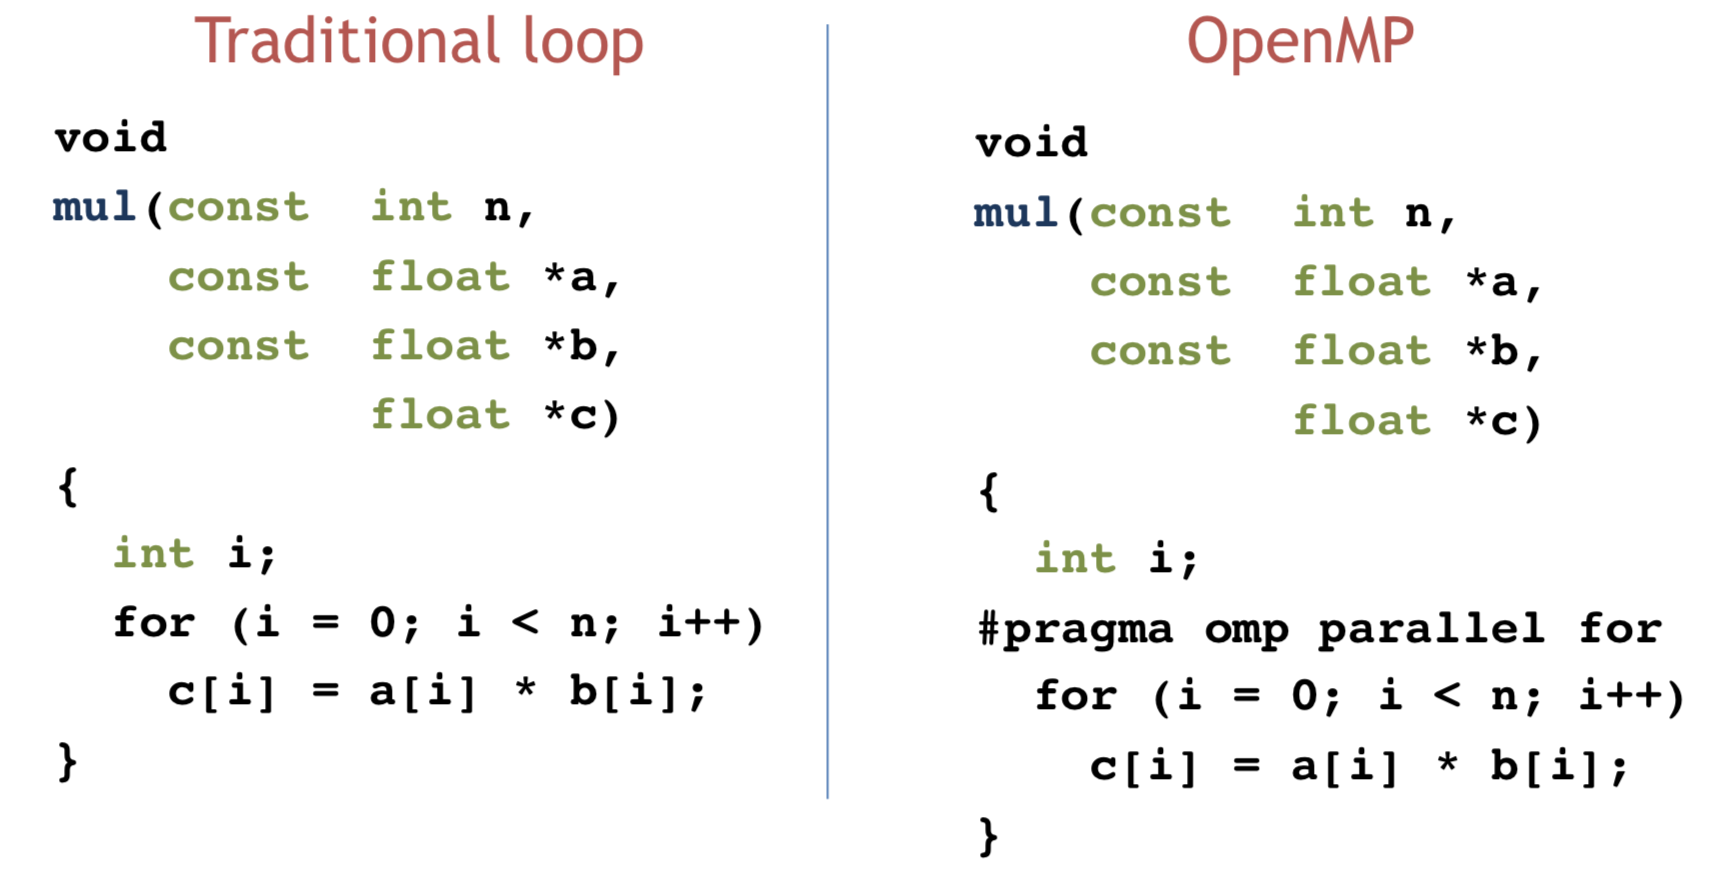
\includegraphics[width=\linewidth]{images/big-idea-behind-opencl.png}
    \caption{The big idea behind OpenCL}
    \label{fig:my_label}
\end{figure}

\subsection{OpenCL Memory model}

\begin{figure}[h]
    \centering
    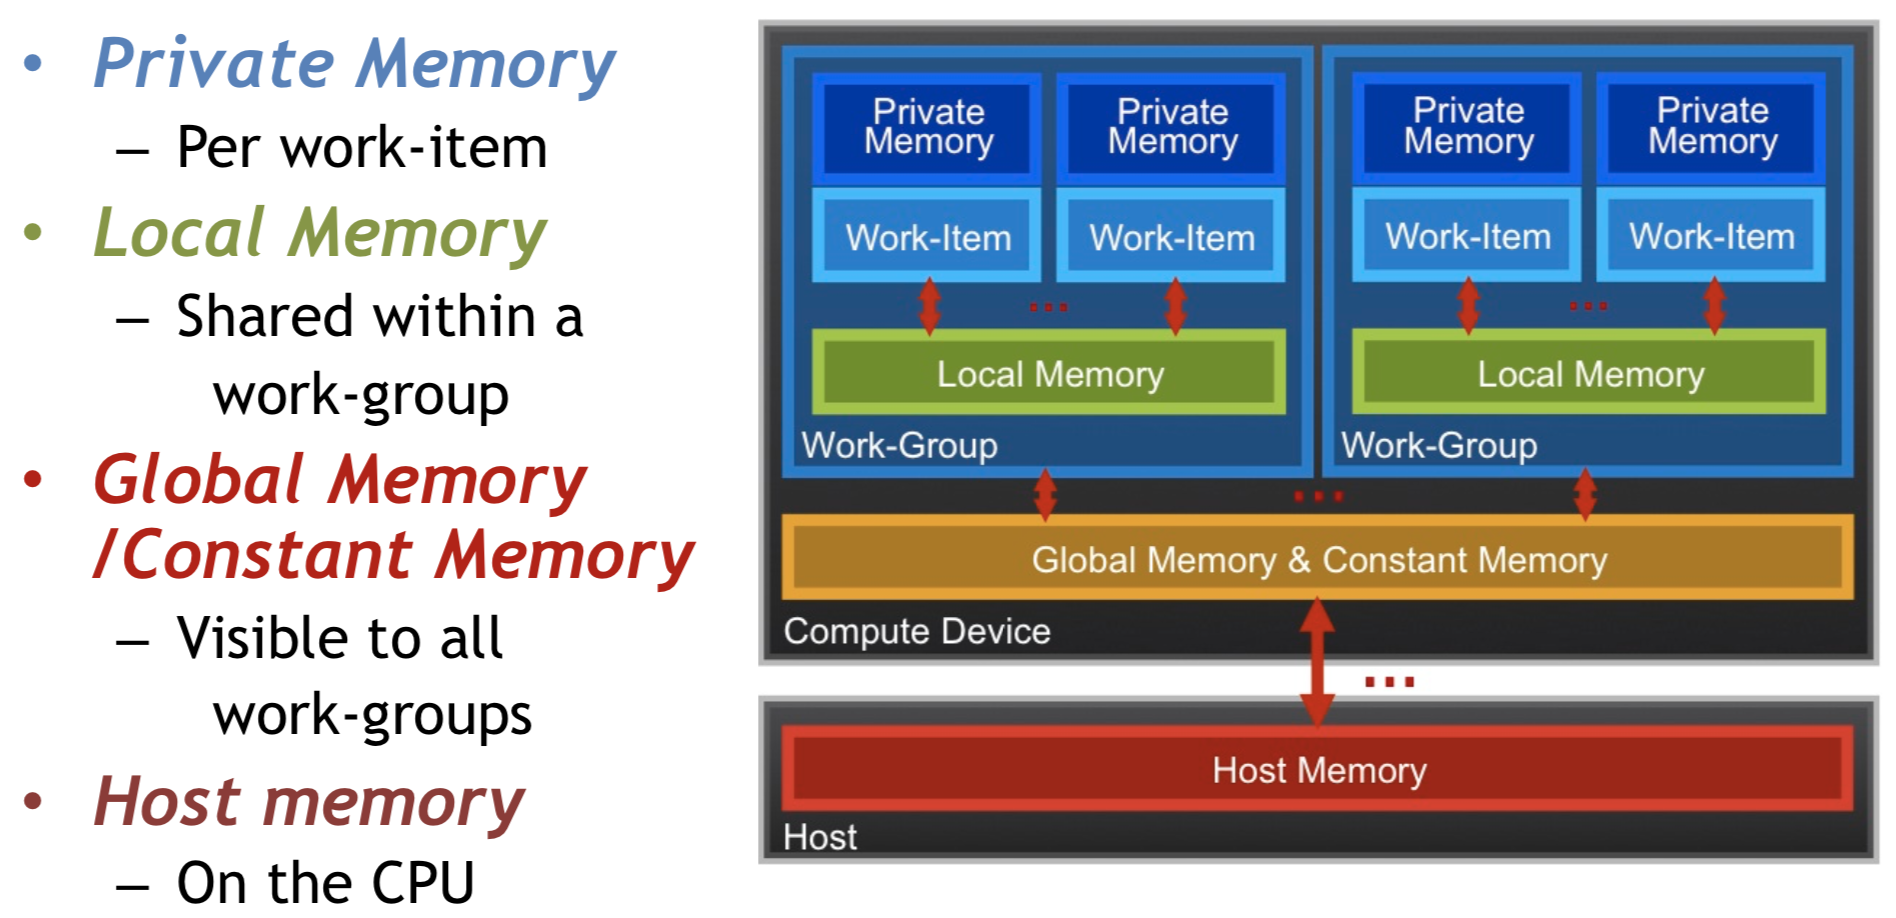
\includegraphics[width=\linewidth]{images/opencl-memory-model.png}
    \caption{OpenCL Memory Model}
    \label{fig:my_label}
\end{figure}


\subsection{Implementation of OpenCL}

OpenCL has two parts, kernel code and host code. For the host code, there are five simple steps: Define the platform, Create and Build the program, Setup memory objects, Define the kernel and Submit commands.

\textbf{Define the platform}

\begin{figure}[h]
    \centering
    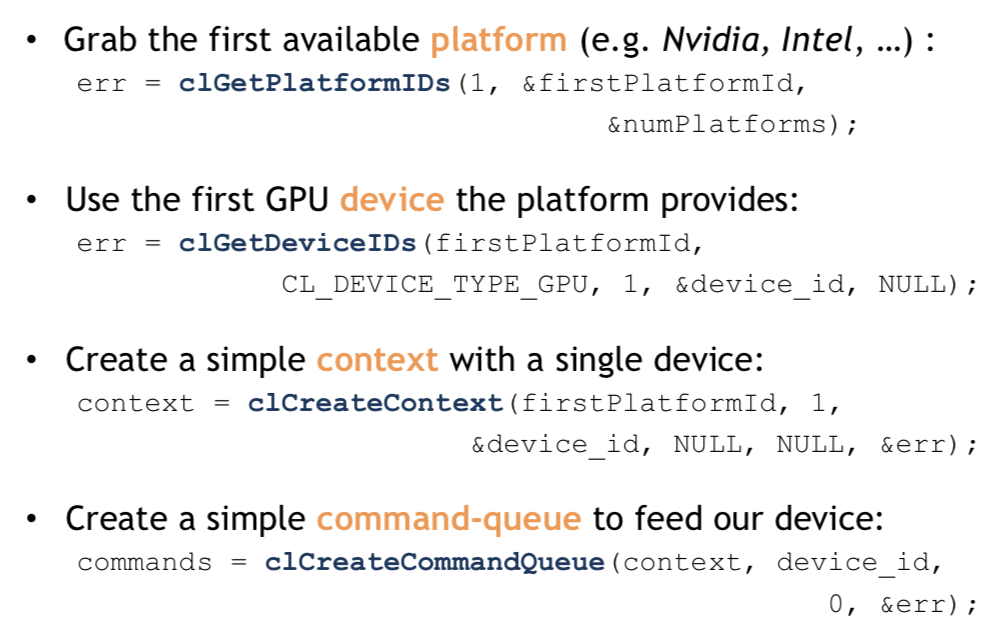
\includegraphics[width=0.8\linewidth]{images/define-the-platform.png}
    \caption{Define the Platform}
    \label{fig:my_label}
\end{figure}


\textbf{Create and Build the program} define the source code for the kernel-program as a string literal or read it from a file.

\begin{figure}[h]
    \centering
    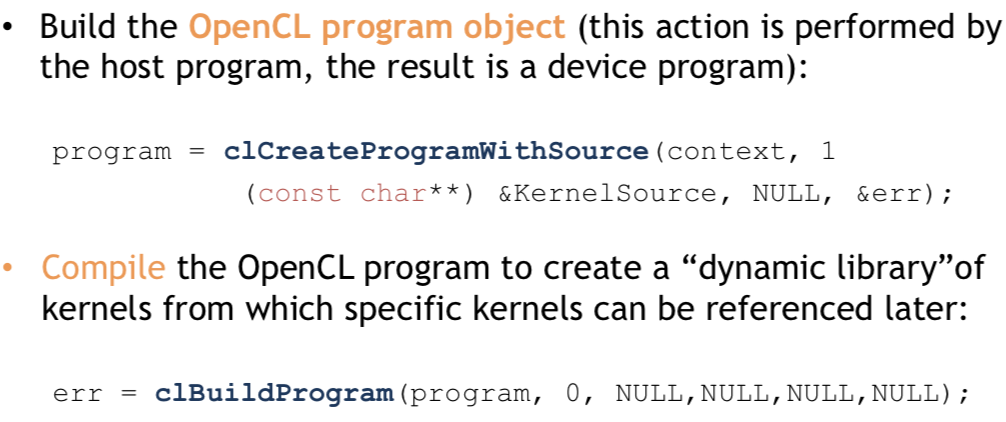
\includegraphics[width=0.8\linewidth]{images/create-and-build-the-program.png}
    \caption{Create and Build the Program}
    \label{fig:my_label}
\end{figure}


\textbf{Setup memory objects}: The buffers are declared on the host as type \textbf{cl\_mem}. It needs arrays in host memory hold the original host-side data.



\begin{figure}[h]
    \centering
    \begin{subfigure}{0.45\textwidth}
    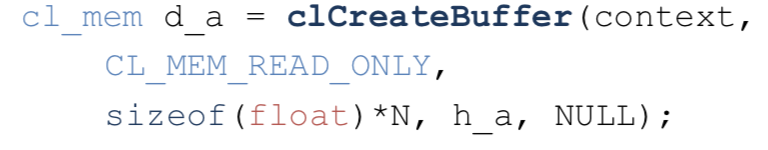
\includegraphics[scale=0.5]{images/create-the-buffer.png}
    \caption{Create the Buffer}
    \label{fig:my_label}
    \end{subfigure}
    \begin{subfigure}{0.45\textwidth}
    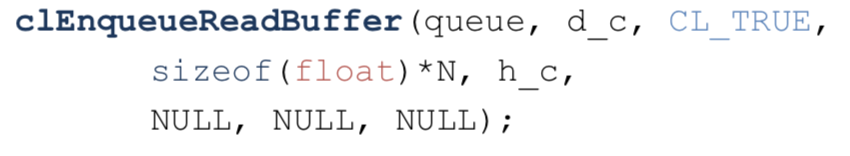
\includegraphics[scale=0.5]{images/set-the-data-to-buffer.png}
    \caption{Set the Data to Buffer}
    \label{fig:my_label}
    \end{subfigure}
\end{figure}


\textbf{Define the kernel}

\begin{figure}[h]
    \centering
    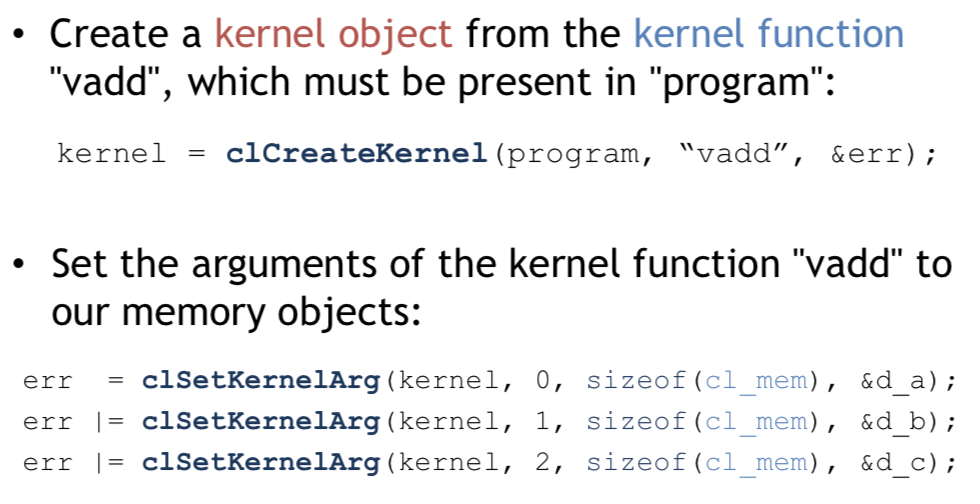
\includegraphics[width=0.8\linewidth]{images/define-the-kernel.png}
    \caption{Define the Kernel}
    \label{fig:my_label}
\end{figure}


\textbf{Enqueue commands}

\begin{figure}[h!]
    \centering
    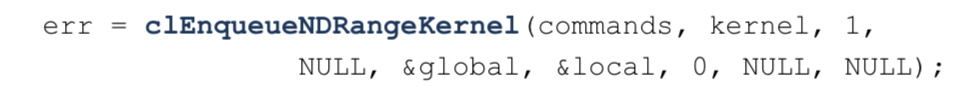
\includegraphics[width=0.8\linewidth]{images/enqueue-commands.png}
    \caption{Enqueue the Commands}
    \label{fig:my_label}
\end{figure}


For the kernel code:

\begin{figure}[h]
    \centering
    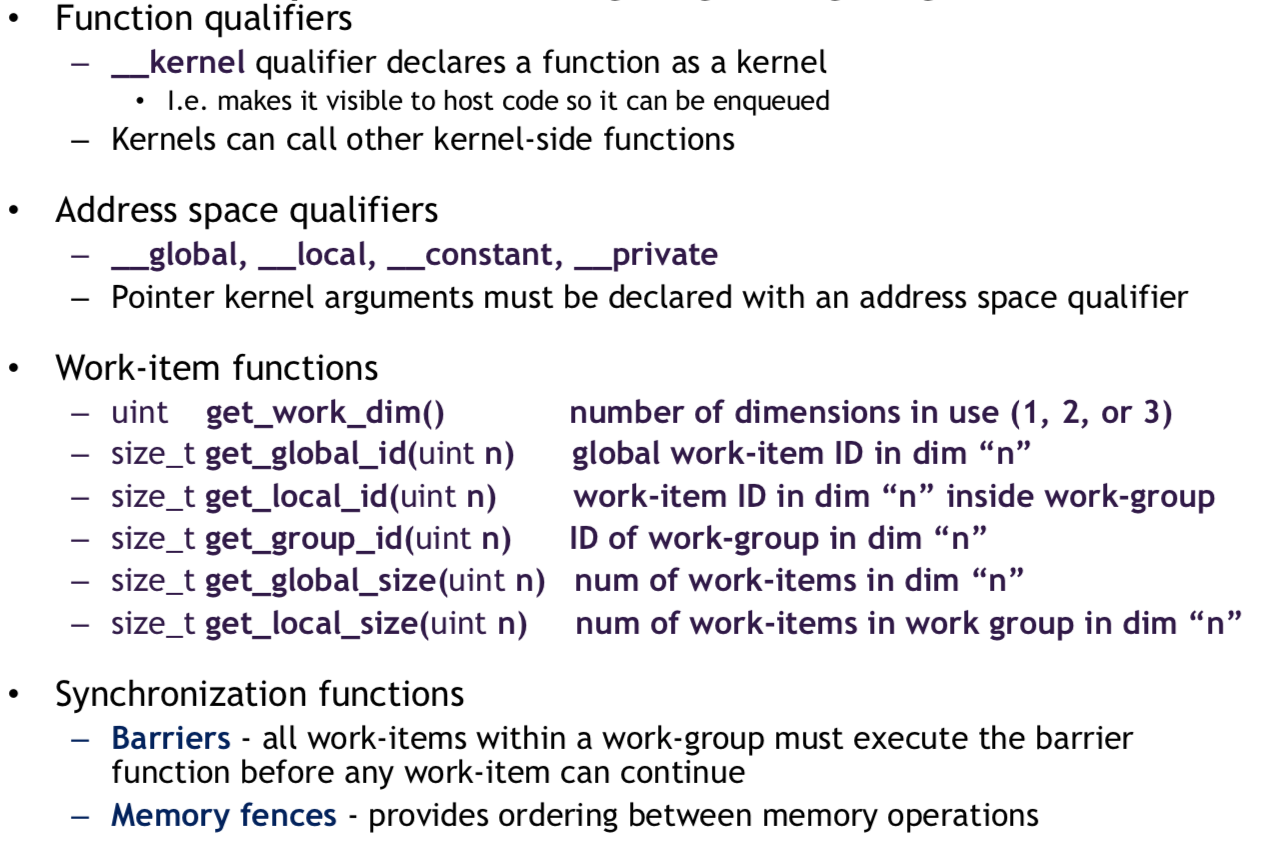
\includegraphics[width=0.8\linewidth]{images/opencl-c-language-restrictions.png}
    \caption{OpenCL C Language Restrictions}
    \label{fig:my_label}
\end{figure}


\subsection{Optimisation of OpenCL}


\textbf{Branching}, GPUs tend not to support speculative execution, which means that branch instructions have high latency.

\begin{figure}[h!]
    \centering
    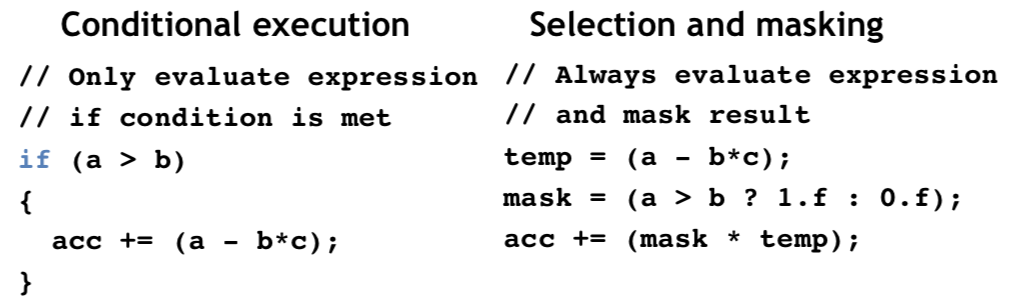
\includegraphics[width=0.5\linewidth]{images/branching.png}
    \caption{Branching}
    \label{fig:my_label}
\end{figure}



\textbf{Memory access patterns}, GPU  prefers  to  access  memory  continuouslyin  successive  work-items.

\begin{figure}[h!]
    \centering
    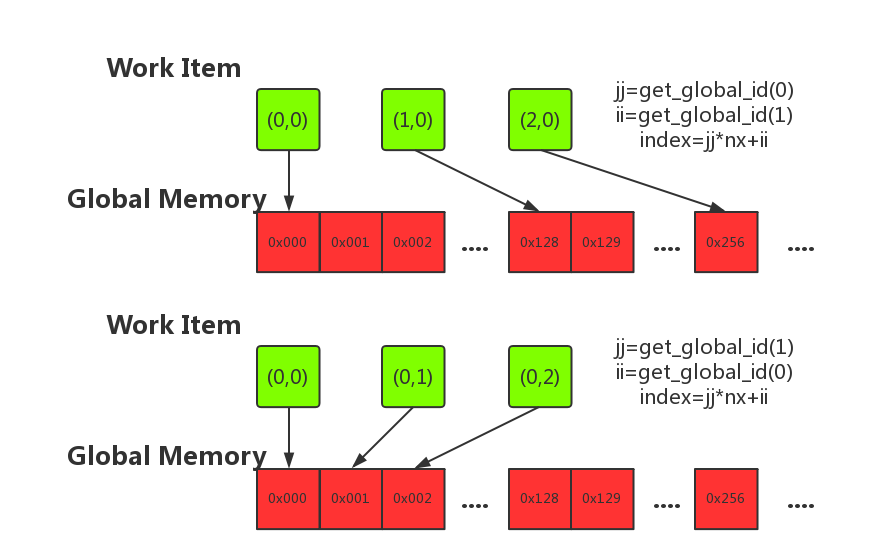
\includegraphics[width=0.5\linewidth]{images/memory-access-patterns.png}
    \caption{Memory Access Patterns}
    \label{fig:my_label}
\end{figure}




\end{document}
